%%% LaTeX Template: Two column article
%%%
%%% Source: http://www.howtotex.com/
%%% Feel free to distribute this template, but please keep to referal to http://www.howtotex.com/ here.
%%% Date: February 2011

%%% Preamble
\documentclass[	DIV=calc,%
							paper=a4,%
							fontsize=12pt,%
							onecolumn]{scrartcl}	 					% KOMA-article class

\usepackage{lipsum}													% Package to create dummy text
\usepackage[english]{babel}										% English language/hyphenation
\usepackage[protrusion=true,expansion=true]{microtype}				% Better typography
\usepackage{amsmath,amsfonts,amsthm}					% Math packages
\usepackage[pdftex]{graphicx}									% Enable pdflatex
\usepackage[svgnames]{xcolor}									% Enabling colors by their 'svgnames'
\usepackage[hang, small,labelfont=bf,up,textfont=it,up]{caption}	% Custom captions under/above floats
\usepackage{epstopdf}												% Converts .eps to .pdf
\usepackage{subfig}													% Subfigures
\usepackage{booktabs}												% Nicer tables
\usepackage{fix-cm}													% Custom fontsizes
\usepackage[utf8]{inputenc}
\usepackage[top=2.5cm, bottom=2.5cm, left=2.5cm, right=2.5cm]{geometry}
\usepackage[ddmmyyyy]{datetime}
\addto\captionsenglish{%
	\renewcommand\tablename{Tabela}
	\renewcommand\figurename{Figura}
} 
 

 
%%% Custom sectioning (sectsty package)
\usepackage{sectsty}													% Custom sectioning (see below)
\allsectionsfont{%															% Change font of al section commands
	\usefont{OT1}{phv}{b}{n}%										% bch-b-n: CharterBT-Bold font
	}

\sectionfont{%																% Change font of \section command
	\usefont{OT1}{phv}{b}{n}%										% bch-b-n: CharterBT-Bold font
	}



%%% Headers and footers
\usepackage{fancyhdr}												% Needed to define custom headers/footers
	\pagestyle{fancy}														% Enabling the custom headers/footers
\usepackage{lastpage}	

% Header (empty)
\lhead{}
\chead{}
\rhead{}
% Footer (you may change this to your own needs)

%% ====================================
%% ====================================
%% mude o rodape  do projeto
%% ====================================
%% ====================================

\lfoot{\footnotesize \texttt{Projeto de Redes} \textbullet Reestruturação do Cabeamento}


\cfoot{}
\rfoot{\footnotesize página \thepage\ de \pageref{LastPage}}	% "Page 1 of 2"
\renewcommand{\headrulewidth}{0.0pt}
\renewcommand{\footrulewidth}{0.4pt}



%%% Creating an initial of the very first character of the content
\usepackage{lettrine}
\newcommand{\initial}[1]{%
     \lettrine[lines=3,lhang=0.3,nindent=0em]{
     				\color{DarkGoldenrod}
     				{\textsf{#1}}}{}}



%%% Title, author and date metadata
\usepackage{titling}															% For custom titles

\newcommand{\HorRule}{\color{DarkGoldenrod}%			% Creating a horizontal rule
									  	\rule{\linewidth}{1pt}%
										}

\pretitle{\vspace{-30pt} \begin{flushleft} \HorRule 
				\fontsize{50}{50} \usefont{OT1}{phv}{b}{n} \color{DarkRed} \selectfont 
				}

%% ====================================
%% ====================================
%% mude o titulo  do projeto
%% ====================================
%% ====================================

\title{Reestruturação de Infraestrutura de Redes}					% Title of your article goes here

%% ====================================



\posttitle{\par\end{flushleft}\vskip 0.5em}

\preauthor{\begin{flushleft}
					\large \lineskip 0.5em \usefont{OT1}{phv}{b}{sl} \color{DarkRed}}
\author{Leandro Tavares, Sidnei Gobetti de Lima }  	% Author name goes here


\postauthor{\footnotesize \usefont{OT1}{phv}{m}{sl} \color{Black} 
					\\Universidade Tecnológica Federal do Paraná - Câmpus Cornélio Procópio 								% Institution of author
					\par\end{flushleft}\HorRule}

\date{}																				% No date




%%% Begin document
\begin{document}
\maketitle
\thispagestyle{fancy} 	
\thispagestyle{empty}		% Enabling the custom headers/footers for the first page 
% The first character should be within \initial{}




%% ====================================
%% ====================================
%% mude o resumo  do projeto
%% ====================================
%% ====================================
\initial{E}\textbf{ste projeto vem propôr uma reestruturação do cabeamento de redes já existente em uma organização fictícia. Buscaremos definir e implantar as melhores práticas nessa nova estruturação, objetivando um melhor desempenho da rede, qualidade de comunicação e assegurar a confiabilidade na troca de informações na rede.}

%% ====================================
\begin{figure}
	\centering
	
\includegraphics{utfpr}
\end{figure}

\vspace{3cm}
\centerline{\textit{\textbf{\today}}}

\clearpage
    \renewcommand*\listfigurename{Lista de figuras}
\listoffigures

\renewcommand*\listtablename{Lista de tabelas}
\listoftables




\clearpage
\renewcommand{\contentsname}{Sumário}
\tableofcontents
\clearpage

%% ====================================
%% ====================================
%% Inicio do texto
%% ====================================
%% ====================================
\section{Introdução}
Será realizado uma reestruturação da rede de uma organização fictícia. Essa empresa atua no ramo alimentício, atendendo as cidades de Cascavel e Curitiba, possuindo um total de 12 filiais distribuídas nessas regiões. Contudo, a reestruturação será realizada apenas em uma filial, situada em Cascavel. Essa filial possui 200 colaboradores atuando em diversas atividades.

O parque de informática dispõe de 50 computadores, 5 servidores físicos, 3 switches, 2 controladores para a rede wireless, bem como impressoras e outros periféricos. A organização possui seu datacenter lotado na cidade de Curitiba, dispondo de vários sistemas, incluindo o sistema de ERP, aonde é acessado por terminal service, por todas as filiais.

Os pontos de venda (PDV) realizam a comunicação diretamente com o servidor em Curitiba. O meio de interconexão utilizado para realizar toda a comunicação entre as filiais e o datacenter é fibra óptica, e a comunição interna por cabeamento de cobre.

A reestruturação proposta para a filial de Cascavel em questão, terá o intuito de readequação da estrutura de rede para certificação. Uma vez que o projeto inicial não atingiu os requisitos para a certificação da estrutura. Outro ponto que será incluído no projeto é a implantação de uma estrutura virtual redundante para servidor de arquivos, pois segue um modelo que não atende a necessidade atual da empresa. 
\subsection{Benefícios}
A reestruturação da infraestrutura de rede trará benefícios impactantes, tais como:
\begin{itemize}
	\item Desempenho da rede melhorado: A eliminação dos gargalos presentes na rede irá aumentar o desempenho da rede, agilizando ainda mais o trafego de dados.
	
	\item Confiabilidade na transferência das informações: Com maior conformidade da infraestrutura, as informações terão maior garantia de entrega ao destino, e assim, aumentando o QoS ( Quality of Service).
	
	\item Menor custo de manutenção: Estando com a rede certificada, o custo com manutenções no cabeamento serão praticamente extintos.
\end{itemize}
Em decorrência disso, colaboradores podem aumentar sua produtividade, pois os problemas existentes devido a interrupção da comunicação, relacionadas a infraestrutura de rede, serão extremamente reduzidas. Os clientes ficarão mais satisfeitos, e dessa forma, os serviços que serão entregues podem agregar maior valor ao negócio. 

Por conta de tudo isso, a organização terá benefícios de curto a longo prazo, principalmente, econômicos.


\section{Estado atual}
Atualmente a infraestrutura de rede possui os seguintes itens:

\begin{itemize}
	\item 1 Rack Piso Fechado 44U x 870mm
	\item 1 Nobreak HDS Maxxi Mono 6KVA
	\item 1 Link de Fibra Óptica Copel 5Mbps FULL (Domínio)
	\item 1 Link de Fibra Óptica Copel 12Mbps FULL (Ocioso)
	\item 1 Link de Internet Vivo 15 Mbps (Clientes)
	\item 2 Fibras Ópticas Monomodo para conexão interna
	\item 2 Converter Gigabit Media Planet GT-805A 10/100/1000Base-T para 1000Base SX/LX
	\item 1 Converter Media Bridge Planet FT-802 10/100Base-TX para 100Base-FX 
	\item 1 Converter Media DNet DN-MCCOP SMSC25WB 10/100Base-Tx para 100Base-FX
	\item 2 Switch 3Com Baseline 2952-SFP plus  10/100/1000- 48 portas - 1Gbit 4 X SFP
	\item 1 Switch 3Com Baseline 2928-SFP plus 10/100/1000 - 24 portas - 1Gbit 4 X SFP
	\item 1 Switch Enterasys SecureStack A2 A2H124 10/100 – 24 portas – 1Gbit 2 X SFP
	\item 3 Switch D-NET DN-SF1024 10/100 - 24 portas 
	\item 1 Switch LG LS3124A 10/100 24 portas 
	\item 2 Wireless Controller Siemens HiPath C20
	\item 15 Wireless Access Point  Siemens HiPath 2610 - IEEE 802.11b,a,g
	\item 1 Access Point Dlink 300Mbps
	\item 2 Roteadores Wireless Tplink TL-WR842ND (exclusive para o TEF) 
	\item 1 Modem DLink DSR-2640B
	\item 1 Access Point Ubiquiti Unifi Uap-Ir Long Range 300Mbps (Clientes e Fornecedores) 
	\item 1 Hub LG 8P
	\item 3 Patch Panels Furukawa - Cat6 - 24 Portas
	\item 1 Patch Panel AMP Interconect – Cat 6 – 24 Portas
	\item 110 Pontos de rede Cat 6
	\item Cabeamento Furukawa Gigalan STD U/UTP Cat6
\end{itemize}

A principal reclamação dos colaboradores é a lentidão do sistema e que constantemente ficam sem acesso a internet ou ao servidor. A comunicação dentro do domínio, inclusive acesso a internet, é realizada utilizando um único link de fibra. Inclusive um link de fibra com acesso a internet que está ocioso no momento.

Visualizando a estrutura, pode-se observar inicialmente que existem cabos sendo ligados aos desktops diretamente, sem a utilização de patch cord. Em alguns casos, patch cords são utilizados, porém, são de padrões diferentes. Dessa forma, não esta sendo seguido o padrão correto, visto que o cabeamento não é flexível.

Outro ponto de preocupação é a distancia que os cabos percorrem dentro da organização. Pois em alguns pontos pode-se verificar que ultrapassa dos 90 metros, visto todo o caminho que os cabos percorrem até seu destino. Podemos identificar ainda, que os cabos podem sofrer interferências, pois em alguns casos passam bem próximos a equipamentos elétricos e eletrônicos de grande porte, como por exemplo, a câmara fria, e até mesmo próximo a uma caixa d’agua, que dificulta a transmissão de sinais wireless.

Existe um caso que está utilizando emenda plástica para um cabo de rede, e isso não deve ocorrer. Outro caso que segue incorretamente é com relação a utilização de um hub para interligar um computador e uma impressora a rede de domínio.

A identificação do cabeamento e dos pontos de rede existe parcialmente, e assim, alguns pontos e cabos possuem identificação e outros não. Isso dificulta possíveis manutenções, devido ao tempo que será atribuído para identificação do problema.

O cascateamento da rede é evidente quando notamos a utilização de muitos switches. Fora do Rack, conseguimos observar 4 switches. Inclusive um roteador wireless sendo conectado a um switch, e em seguida ligado a outro roteador wireless. 


\section{Usuários e Aplicativos}
Do quadro total de funcionários presentes na organização, atualmente conta com 70 usuários ativos, que possuem acesso a um dos sistema utilizados. A empresa está em crescimento de vendas, contudo, não existe tendência em aumentar o número de usuários. Consequentemente, pontos de redes já existentes poderão ser eliminados ou remanejados.

Com relação aos equipamentos, existe uma necessidade para aumentar a disponibilidade de serviços e a qualidade da internet para clientes. Assim, será necessário realizar um levantamento dos equipamentos que poderão ser utilizados para suprir essa necessidade.

 

\subsection{Usuários}
Conforme já mencionado anteriormente, a organização possui 70 usuários ativos. Grande parte desses colaboradores são jovens, entre 18 a 24 anos, e utilizam principalmente o sistema de vendas no PDV (Ponto de Venda).

Os outros colaboradores, utilizam o software de ERP. O software utilizado é acessado por conexão via Terminal Service. Os usuários desse software, são funcionários que já utilizaram o sistema de vendas em algum momento anterior, e possuem portanto maior tempo de experiência dentro da organização.


\subsection{Aplicativos}
Os serviços e aplicativos necessários atualmente para que o negócio mantenha-se em funcionamento foram separados em Serviços Críticos e Aplicativos Críticos, e serão descritos abaixo:
\begin{itemize}
	\item SERVIÇOS CRÍTICOS
	
		1 - Acesso à Internet/intranet: O acesso a rede internet/intranet é fundamental para realização da comunicação entre os pontos de venda e o servidor central em Curitiba, e também, na comunicação com o software ERP;
		
		2 - DHCP: Alguns dispositivos estão configurados para receber automaticamente endereçamento do servidor de DHCP;
		
		3 - E-mail: Fornecedores, clientes e colaboradores se comunicam constantemente pelo email corporativo, dessa forma é necessários estar sempre ativo;
		
		4 - Servidor de Arquivos: Cada colaborador pode armazenar seus arquivos que julga importante nesse servidor, e assim, ter uma cópia salva em local seguro.
		
	\item APLICATIVOS CRÍTICOS
	
		1 - Sistema de Vendas : Cada ponto de venda possui instalado o sistema de vendas em seu hard disk, que comunica por meio da rede com a central em Curitiba. Um desastre envolvendo esse sistema, impossibilita totalmente a operação da empresa;
		
		2 - Sistema de Transferência Eletrônica de Fundo (TEF): Responsável pela efetivação dos pagamentos por cartão de crédito e débito. Sua paralização trás péssimos resultados para a organização, visto que uma quantidade expressiva dos pagamentos são realizados utilizando cartão;
		
		3 - Sistema de Enterprise Resource Planning (ERP): Realiza todo o controle fiscal, estoque, financeiro. Assim, sua indisponibilidade pode atingir todos os colaboradores da empresa, inclusive clientes.
		
\end{itemize}


\section{Estrutura predial existente}


A estrutura predial da organização é exibida logo abaixo pela Figura \ref{Fig_estrutura_predial}.

\begin{figure}[h!]
	\centering
	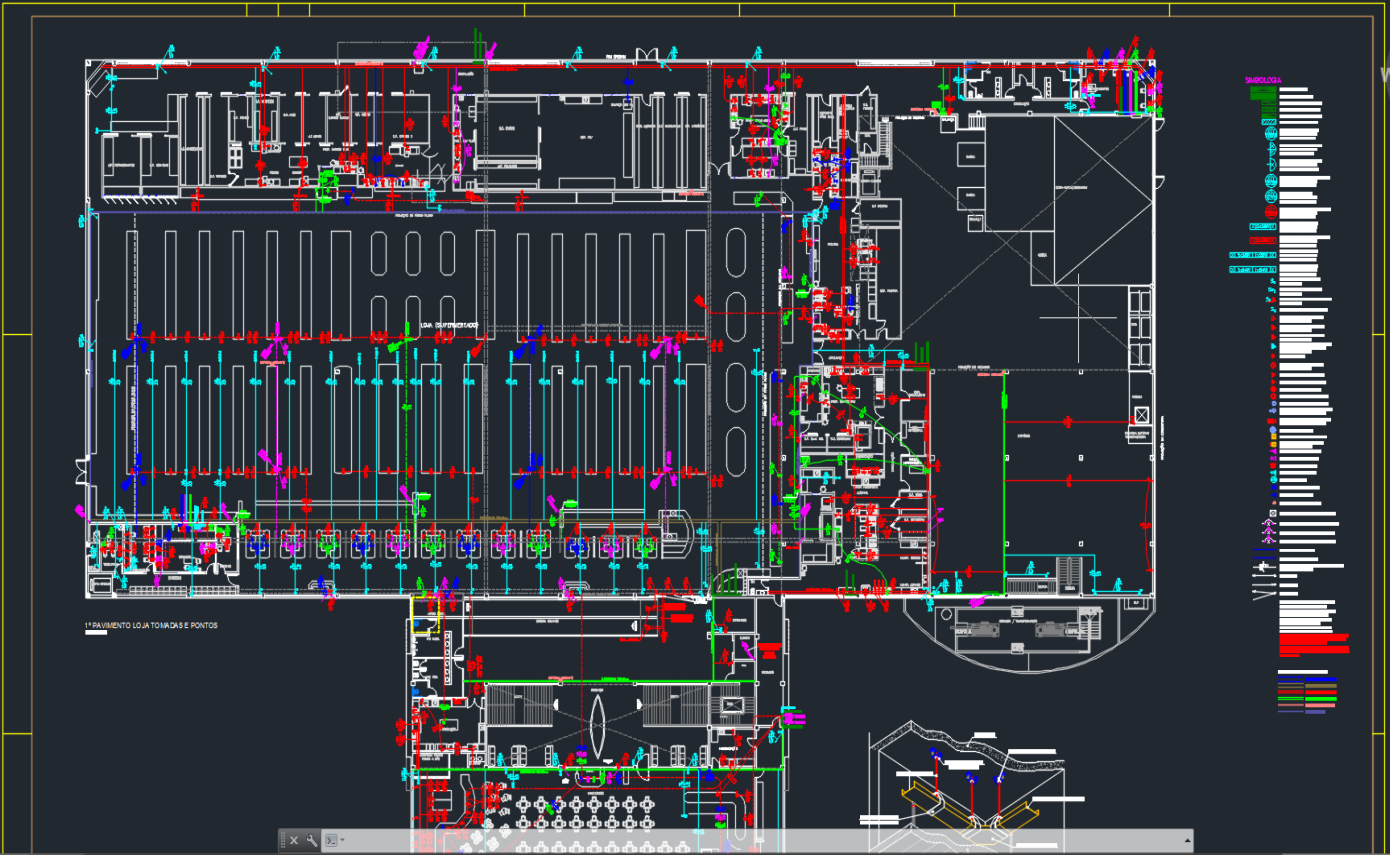
\includegraphics[width=\textwidth]{Fig_estrutura_predial}
	\caption{Imagem da planta física da empresa}
	\label{Fig_estrutura_predial}
\end{figure}

A infraestrutura da rede cabeada, esta distribuída através de eletrocalhas.  

\begin{itemize}
	
	\item Existe uma eletrocalha principal que segue toda extremidade do prédio, que sai do setor de CPD. Esta eletrocalha possui a largura de 30Cm.
	\item A eletrocalha  principal fica em lugar estratégico, onde há maior concentração dos pontos de redes.
	\item Pontos mais distantes da eletrocalha principal, são levadas através de eletrocalhas menores de 10cm de largura.
	\item A chegada final até o ponto de rede é feita através de conduítes, e tem pontos que chegam com RJ macho direto e outros com pontos RJ fêmea.

\end{itemize}

\section{Planta Lógica - Elementos estruturados}


\subsection{Topologia}


A proposta para a nova infraestrutura abordará inicialmente a alteração do caminho por onde a eletrocalha passa, para evitar a interferência causada por agentes externos. Os cabos que possuírem encaminhamento maior que 90 metros serão realocados em um switch mais próximo, bem como os cabos que possuem emendas.

Todo o cabeamento da organização será padronizado em conforme norma EIA/TIA 568-A. Assim, serão refeitos todos os conectores RJ45 fêmea. Para interligar os hosts aos conectores RJ45 fêmea, bem como os patch panels aos switchs, serão adquiridos patch cords já certificados.

O cascateamento existente será eliminado, realizando um novo encaminhamento de cabos, e assim os hubs serão descartados.

Para aumentar o desempenho da rede, os switchs com velocidade de até 100Mbit serão substituídos por switchs de 1Gbit.

Com o objetivo de aumentar a disponibilidade da internet, será ativado o link de fibra já existente.

Após isso, será realizada a identificação do cabeamento e dos pontos de rede existentes e também dos que serão incluídos.

Por fim, realizaremos a certificação da rede, e dessa forma, evitar possíveis problemas relacionados a infraestrutura de rede.





\begin{figure}[h!]
	\centering
	\includegraphics[width=9cm,height=9cm,keepaspectratio]{DiagramaTopologiaRede}
	\caption{Topologia lógica da rede}
	\label{DiagramaTopologiaRede}
\end{figure}


Continuar explicação figura \ref{DiagramaTopologiaRede}

\subsection{Encaminhamento}



O encaminhamento dos cabos é realizado por meio de eletrocalhas e eletrodutos. A eletrocalha principal que segue por todo o comprimentos da edificação, fornece suporte para a passagem do cabeamento, bem como suas ramificações. Ela mede 30cm de largura, as ramificações possuem 20cm de largura e leva os cabos até os setores. As eletrocalhas são pré zincadas, pois não estão sujeitas a grande ocorrência de corrosão. Chegando no setor, o cabo segue para o ponto de rede por meio de um eletroduto.




\subsection{Memorial descritivo}

Relacione todos os equipamentos passivos que serão utilizados, tipo, fabricante, quantidade.

\subsection{Identificação dos cabos}

\section{Implantação}
Estabeleça um cronograma de implantação:
Remoção de equipamentos existentes (destino para descarte), instalação dos condutores, instalação dos cabos, 
identificação dos cabos, montagem dos racks, certificação, etc... Crie atividades e estabeleça o tempo de execução. Se for um projeto real, indique também quais os responsáveis pela execução do projeto e de cada uma das etapas.

Defina marcas (e padrões) e fornecedores se for o caso. Atenção a contratados e subcontratados para a realização das atividades. Estabeleça a responsabilidade de execução da atividade e também da validação dela.

Utilize algum software para gerear o cronograma. Excel,etc. O fundamental é dividir em etapas, descrever e estimar o tempo de cada uma delas.

Segue uma relação de ferramentas:
http://asana.com/, 
https://trello.com/, 
http://www.ganttproject.biz/, 
http://www.orangescrum.org/. 

\section{Plano de certificação}
Quais seriam as etapas para a certificação? 
Quais os locais e horários para execução da certificação na rede? Toda rede será certificada?
Como os testes seriam executados?
Quais relatórios de certificação serão (ou deveriam ser) entregues? 

\section{Plano de manutenção}

Revisões periódicas na rede, emissão de certificados para novos pontos.

\subsection{Plano de expansão}
Existe um plano de expansão? Quantos novos pontos poderão ser acrecidos na rede, antes de migração de equipamentos na camada 2? Se houver expansão, quais equipamentos deverão ser direcionados para as estremidades da rede? 


\section{Orçamento}
Crie uma relação de orçamentos baseado na seções anteriores.

\section{Referências bibliográficas}
Utilize o mendley, o jabref ou diretamente o bibtex para gerenciar suas referências biliográficas. As referências são criadas automaticamente de acordo com o uso no texto.

Exemplo: Redes de computadores, segundo \cite{t2013} é considerada..... Já \cite{kurose2010} apresenta uma versão...

Analisando os pressupostos de \cite{ref3} e \cite{ref4} concluimos que....


\renewcommand\refname{} %%Referências bibliográficas}  
\bibliographystyle{ieeetr}
\bibliography{referencias}  

%% ***********************************************************************
%% === remover daqui =====================================================
%% ***********************************************************************
..
%% ***********************************************************************
%% === ate aqui    =====  ================================================
%% ***********************************************************************
\end{document}